\documentclass[tikz,border=2pt]{standalone}
\usepackage{amsmath,amssymb}
\usepackage{tikz}

\begin{document}
% A partition chops S into pieces that do not overlap and together cover everything:
% exactly one of the B_i happens.
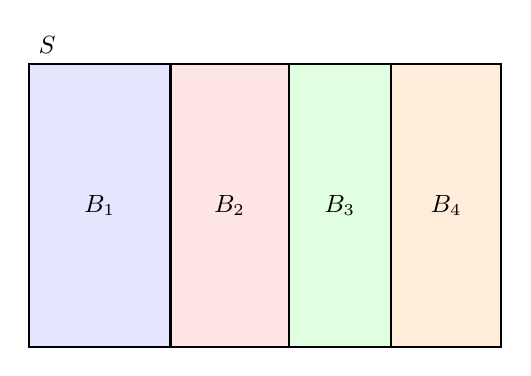
\begin{tikzpicture}[every node/.style={font=\small}]
	\fill[blue!10] (-3,-1.8) rectangle (-1.2,1.8);
	\fill[red!10] (-1.2,-1.8) rectangle (0.3,1.8);
	\fill[green!12] (0.3,-1.8) rectangle (1.6,1.8);
	\fill[orange!15] (1.6,-1.8) rectangle (3,1.8);
	\draw[thick] (-3,-1.8) rectangle (3,1.8);
	\draw[thick] (-1.2,-1.8) -- (-1.2,1.8);
	\draw[thick] (0.3,-1.8) -- (0.3,1.8);
	\draw[thick] (1.6,-1.8) -- (1.6,1.8);
	\node at (-2.1,0) {$B_1$};
	\node at (-0.45,0) {$B_2$};
	\node at (0.95,0) {$B_3$};
	\node at (2.3,0) {$B_4$};
	\node[anchor=south west] at (-3,1.8) {$S$};
	
\end{tikzpicture}
\end{document}
